\documentclass[12pt,reqno]{amsart}

%\usepackage[notcite,notref]{showkeys}
\usepackage{tikz, tikz-cd}
\usepackage{bbm,bm}
\usepackage[utf8]{inputenc}
\usepackage[T1]{fontenc}
\usepackage[english]{babel}
%\usepackage{rotating}
%\usepackage{newpxtext,newpxmath} % The Palantino font, it includes amssymb. 
\usepackage{amsmath, amsthm}
\usepackage{amssymb} 
\usepackage{comment}
%\usepackage[all]{xy}
\usepackage{todonotes}
\usepackage{caption}
\usepackage{mathtools}
\usepackage{sidecap}
\usepackage{subcaption}
\usepackage{xcolor}
%\usepackage{subfig, subfigure}


\setlength{\parindent}{0pt}
\sloppy
\flushbottom

\usepackage{color}
\newcommand{\blue}[1]{\textcolor{blue}{#1}}
\newcommand{\red}[1]{\textcolor{red}{#1}}
\newcommand{\green}[1]{\textcolor{green}{#1}}

\usepackage[bookmarks=false,colorlinks,linkcolor=blue,citecolor=red]{hyperref}
%%---- page geometry & headings
%%%%%%%%%%%%%%%%%%%%%%%%%%%%%%%% 
\addtolength{\textheight}{48pt}
\addtolength{\voffset}{-24pt}
\addtolength{\textwidth}{86pt}
\addtolength{\hoffset}{-42pt}
%%%%%%%%%%%%%%%%%%%%%%%%%%%%%%%%

\pagestyle{headings} % empty}

\date{\today}


%-------------------------------------------------------------------
% ENVIRONMENTS
%-------------------------------------------------------------------
\theoremstyle{plain}
\newtheorem{theorem}{Theorem}[section]
\newtheorem{corollary}[theorem]{Corollary}
\newtheorem{lemma}[theorem]{Lemma}
\newtheorem{proposition}[theorem]{Proposition}
\newtheorem{conjecture}[theorem]{Conjecture}
%\numberwithin{theorem}{subsection} use this, if we want to number theorems, etc. by subsections x.x.x

\theoremstyle{definition}
\newtheorem{example}[theorem]{Example} 
\newtheorem{remark}[theorem]{Remark} 
\newtheorem{definition}[theorem]{Definition} 
%\theoremstyle{remark}
\newtheorem*{associativity}{Associativity}
%\newtheorem*{unitality}{Unitality}
%\newtheorem*{naturality}{Naturality}
\newtheorem*{compatibility}{Compatibility}
%\newtheorem*{connectedness}{Connectedness}
%\newtheorem*{multiplicativity}{Multiplicativity}
%\newtheorem*{warning}{Warning}
 
 
% TO SEE SPECIAL COMMENT "uncomment" the line bellow
% make sure that "\excludecomment{moredetails}" is the "commented" 
% TO HIDE SPECIAL COMMENT do the opposite as above
\specialcomment{moredetails}{\begingroup\color{red}}{\endgroup}
%\excludecomment{moredetails}


% SET: I,J,K,L
% Set composition:  A,B,C,D
% Parts O,P,Q,R,T,E,F

%-------------------------------------------------------------------
% MACROS
%-------------------------------------------------------------------
% Mathematical Symbols
\DeclarePairedDelimiter\Floor\lfloor\rfloor
\DeclarePairedDelimiter\Ceil\lceil\rceil
\DeclareMathOperator{\spn}{span}
\DeclareMathOperator{\la}{\langle}
\DeclareMathOperator{\ra}{\rangle}
\DeclareMathOperator{\R}{\mathbb{R}}
\DeclareMathOperator{\C}{\mathbb{C}}
\DeclareMathOperator{\F}{\mathbb{F}}
\DeclareMathOperator{\K}{\mathbb{K}}
\DeclareMathOperator{\Z}{\mathbb{Z}}
\DeclareMathOperator{\N}{\mathbb{N}}


\newcommand{\draftnote}[1]{\marginpar{\raggedright\textsf{\hspace{0pt}\red{#1}}}}


\def\field{\Bbbk}
\def\quobasis{\mathcal{G}}
\def\ideal{\langle y_1 + y_2 + \dots + y_n, y^2_1, y^2_2, \dots , y^2_n \rangle}

\newcommand{\xavier}[1]{\todo[color=orange!30]{#1 \\ \hfill --- X.}}
\newcommand{\nantel}[1]{\todo[color=red!30]{#1 \\ \hfill --- N.}}
\newcommand{\vedarth}[1]{\todo[color=blue!30]{#1 \\ \hfill --- V.}}
\setlength{\marginparwidth}{2cm}

\newcommand\catalannumber[3]{
  % start point, size, Dyck word (size x 2 booleans)
  \fill[red!25]  (#1) rectangle +(#2,#2);
  \fill[fill=cyan!60]
  (#1)
  \foreach \dir in {#3}{
    \ifnum\dir=0
    -- ++(0,1)
    \else
    -- ++(1,0)
    \fi
  } |- (#1);
  \draw[help lines] (#1) grid +(#2,#2);
  \draw[dashed] (#1) -- +(#2,#2);
  \coordinate (prev) at (#1);
  \foreach \dir in {#3}{
    \ifnum\dir=0
    \coordinate (dep) at (0,1);
    \else
    \coordinate (dep) at (1,0);
    \fi
    \draw[line width=2pt] (prev) -- ++(dep) coordinate (prev);
  };
}


\newcommand\myfigone[5]{
  % start point, size, Dyck word (size x 2 booleans)
  \fill[red!25]  (#1) rectangle +(#2,#2);
  \fill[fill=cyan!50]
  (#1)
  \foreach \dir in {#3}{
    \ifnum\dir=0
    -- ++(0,1)
    \else
    -- ++(1,0)
    \fi
  } |- (#1);
  \draw[help lines] (#1) grid +(#2,#2);
  \draw[solid, semithick] (#1) -- +(#2,#2);
  \coordinate (prev) at (#1);
  \foreach \dir in {#3}{
    \ifnum\dir=0
    \coordinate (dep) at (0,1);
    \else
    \coordinate (dep) at (1,0);
    \fi
    \draw[draw = red, line width=2pt] (prev) -- ++(dep) coordinate (prev);
  };
  \draw[draw=green!60, very thick] (0, #4 * 2) -- (#4,#4) -- (#4 * 2, 0);
  \node at (0, #4 + 2) [circle, fill = green!60, scale=0.6]{$L_k$};
  \draw[draw=blue!40, very thick] (0, #4 * 2 + 1) -- (#5,#5-1) -- (#4 * 2 + 1, 0);
  \node at (0, #5 + 2) [circle, fill = blue!40, scale=0.6]{$L_d$};
  \draw[densely dashed, thick, draw=red] (#5, #5-1) -- (#5, #2); % dotted lines
  \node at (#5, #5-1) [circle, fill=blue!40, scale=0.3]{}; % blue dot
  \node at (#4, #5-1) [circle, fill=green!60, scale=0.3]{}; % green dot
}

\newcommand\palpha[5]{
  % start point, size, Dyck word (size x 2 booleans)
  \fill[red!25]  (#1) rectangle +(#2 + 1,#2 + 1);
  \fill[fill=cyan!50]
  (2,0)
  \foreach \dir in {#3}{
    \ifnum\dir=0
    -- ++(0,1)
    \else
    -- ++(1,0)
    \fi
  } |- (2,0);
  \draw[help lines] (#1) grid +(#2 + 1,#2 + 1);
  \draw[solid, semithick] (2,0) -- +(#2-1,#2-1);
  \coordinate (prev) at (2,0);
  \foreach \dir in {#3}{
    \ifnum\dir=0
    \coordinate (dep) at (0,1);
    \else
    \coordinate (dep) at (1,0);
    \fi
    \draw[draw = red, line width=2pt] (prev) -- ++(dep) coordinate (prev);
  };


  \path [name path = Ld, draw=blue!40, very thick] (7-4, 8) -- (7,4) -- (8, 3); %L_d line
  \node at (7-4, 8) [circle, fill = blue!40, scale=0.8]{$L_d$}; %L_d text

  \path[name path = Lk, draw=green!60, very thick] (0, 8) -- (4,4) -- (8, 0); %L_k line
  \node at (0, 8) [circle, fill = green!60, scale=0.8]{$L_k$}; %L_k line

  

  \draw[draw=violet, very thick, dashed] plot [smooth] coordinates {(2,0) (2, 1.5)  (2.5, 1.5) (2.5, 2) (3.2, 2.5)};
  %\draw[draw=violet, very thick, dashed] (2,0) -- (2, 1.5) -- (2.2, 1.5) -- (2.2, 4); % dashed straight beta line
  
  % dashed curved beta lines:
  \draw[draw=violet, very thick, dashed, -to] plot [smooth] coordinates {(2.2,4) (2, 5) (2,6)};
  \draw[draw=violet, very thick, dashed] plot [smooth] coordinates {(2.2,4) (3, 4.8) (4,5)};
  \draw[draw=violet, very thick, dashed] plot [smooth] coordinates {(2.2,4) (3, 4.8) (4,5)};
  \draw[draw=violet, very thick, dashed] plot [smooth] coordinates {(2.2,4) (3.5, 4.3) (5,4)};

  

  
  \node at (3, 6) [circle, fill=violet, scale=0.3]{};
  \node at (4, 5) [circle, fill=violet, scale=0.3]{};
  \node at (5, 4) [circle, fill=violet, scale=0.3]{};

  \draw[draw=violet, very thick] (3,6) -- (3,7);
  \draw[draw=violet, very thick] (4,5) -- (4,6);
  \draw[draw=violet, very thick] (5,4) -- (5,5);

  \draw[draw=violet, very thick, dashed] plot [smooth] coordinates {(3,7) (3.1, 7.5) (4,7)};

  %\draw[draw=violet, very thick, dashed] plot [smooth] coordinates {(2.5,4) (3, 4.8) (2,5)};
  %\draw[draw=green!60, very thick] (3-2, 6-2) -- (6-2,3-2) -- (7-2, 2-2);
  %\node at (0, #4 + 2) [circle, fill = green!60, scale=0.8]{$L_k$};
  
  %\draw[densely dashed, semithick] (#5, #5-1) -- (#5, #2); % dotted lines
  %\node at (#5, #5-1) [circle, fill=blue!40, scale=0.3]{}; % blue dot
  %\node at (#4, #5-1) [circle, fill=green!60, scale=0.3]{}; % green dot
}

\newcommand\palphak[5]{
  % start point, size, Dyck word (size x 2 booleans)
  \fill[red!25]  (#1) rectangle +(#2,#2+1);
  \fill[fill=cyan!50]
  (#1)
  \foreach \dir in {#3}{
    \ifnum\dir=0
    -- ++(0,1)
    \else
    -- ++(1,0)
    \fi
  } |- (#1);
  \draw[help lines] (#1) grid +(#2,#2+1);
  \draw[solid, semithick] (#1) -- +(#2,#2);
  \coordinate (prev) at (#1);
  \foreach \dir in {#3}{
    \ifnum\dir=0
    \coordinate (dep) at (0,1);
    \else
    \coordinate (dep) at (1,0);
    \fi
    \draw[draw = black!30!green, line width=2pt] (prev) -- ++(dep) coordinate (prev);
  };
 
  \draw[draw = blue!100,  ultra thick] (1,2) -- (1,3); % k line
  \draw[draw = black!30!green, dashed, ultra thick] (2,3) -- (3,6); % path dashed line
  \draw[draw=red,densely dashed, very thick] (#5, #5-1) -- (#5, #2+1); % dotted lines
  \node at (4, 1) [rectangle, fill = black!30!green, scale=0.7]{$\beta = $\texttt{010\textcolor{blue!100}{0}1}$\cdots$};

}

\newcommand\palphakk[5]{
  % start point, size, Dyck word (size x 2 booleans)
  \fill[red!25]  (#1) rectangle +(#2,#2+ 1);
  \fill[fill=cyan!50]
  (#1)
  \foreach \dir in {#3}{
    \ifnum\dir=0
    -- ++(0,1)
    \else
    -- ++(1,0)
    \fi
  } |- (#1);
  \draw[help lines] (#1) grid +(#2,#2+1);
  \draw[solid, semithick] (#1) -- +(#2,#2);
  \coordinate (prev) at (#1);
  \foreach \dir in {#3}{
    \ifnum\dir=0
    \coordinate (dep) at (0,1);
    \else
    \coordinate (dep) at (1,0);
    \fi
    \draw[draw = black!30!green, line width=2pt] (prev) -- ++(dep) coordinate (prev);
  };
 
  \draw[draw = blue!100,  ultra thick] (1,2) -- (1,3); % k line
  \draw[draw = black!30!green, dashed, ultra thick] (1,4) -- (3,6); % path dashed line
  \draw[draw=red,densely dashed, very thick] (#5-1, #5-2) -- (#5-1, #2+1); % dotted lines
  \node at (4, 1) [rectangle, fill = black!30!green, scale=0.7]{$\beta = $\texttt{010\textcolor{blue!100}{0}0}$\cdots$};

}
\newcommand\palphakkk[5]{
  % start point, size, Dyck word (size x 2 booleans)
  \fill[red!25]  (#1) rectangle +(#2,#2+ 1);
  \fill[fill=cyan!50]
  (#1)
  \foreach \dir in {#3}{
    \ifnum\dir=0
    -- ++(0,1)
    \else
    -- ++(1,0)
    \fi
  } |- (#1);
  \draw[help lines] (#1) grid +(#2,#2+1);
  \draw[solid, semithick] (#1) -- +(#2,#2);
  \coordinate (prev) at (#1);
  \foreach \dir in {#3}{
    \ifnum\dir=0
    \coordinate (dep) at (0,1);
    \else
    \coordinate (dep) at (1,0);
    \fi
    \draw[draw = black!30!green, line width=2pt] (prev) -- ++(dep) coordinate (prev);
  };
 
  \draw[draw = blue!100,  ultra thick] (0,3) -- (0,4); % k line
  \draw[draw = black!30!green, dashed, ultra thick] (1,4) -- (3,6); % path dashed line
  \draw[draw=red,densely dashed, very thick] (#5, #5-1) -- (#5, #2+1); % dotted lines
  \node at (4, 1) [rectangle, fill = black!30!green, scale=0.7]{$\beta = $\texttt{000\textcolor{blue!100}{0}1}$\cdots$};

}
\newcommand\palphakkkk[5]{
  % start point, size, Dyck word (size x 2 booleans)
  \fill[red!25]  (#1) rectangle +(#2,#2+ 1);
  \fill[fill=cyan!50]
  (#1)
  \foreach \dir in {#3}{
    \ifnum\dir=0
    -- ++(0,1)
    \else
    -- ++(1,0)
    \fi
  } |- (#1);
  \draw[help lines] (#1) grid +(#2,#2+1);
  \draw[solid, semithick] (#1) -- +(#2,#2);
  \coordinate (prev) at (#1);
  \foreach \dir in {#3}{
    \ifnum\dir=0
    \coordinate (dep) at (0,1);
    \else
    \coordinate (dep) at (1,0);
    \fi
    \draw[draw = black!30!green, line width=2pt] (prev) -- ++(dep) coordinate (prev);
  };
 
  \draw[draw = blue!100,  ultra thick] (0,3) -- (0,4); % k line
  \draw[draw = black!30!green, dashed, ultra thick] (0,5) -- (3,6); % path dashed line
  \draw[draw=red,densely dashed, very thick] (#5-1, #5-2) -- (#5-1, #2+1); % dotted lines
  \node at (4, 1) [rectangle, fill = black!30!green, scale=0.7]{$\beta = $\texttt{000\textcolor{blue!100}{0}0}$\cdots$};

}

%%%%%%%%%%%%%%
%%  TITLE AND AUTHORS
%%%%%%%%%%%%%%


\author{Nantel Bergeron}\address[Bergeron]
{Department of Mathematics and Statistics\\ York  University\\ To\-ron\-to, Ontario M3J 1P3\\ CANADA}
\email{bergeron@mathstat.yorku.ca}
\urladdr{http://www.math.yorku.ca/bergeron}

\author{Xavier Mootoo}\address[Mootoo]
{Department of Mathematics and Statistics\\ York  University\\ To\-ron\-to, Ontario M3J 1P3\\ CANADA}
\email{xmootoo@gmail.com}



\thanks{Bergeron: Research supported in part by NSERC and York Research Chair.}
\thanks{Mootoo: Research supported by NSERC and York University}


\title[{G}r\"obner Basis for a Symmetric Function Ideal]{{C}onstructing a Gr\"obner Basis of a Symmetric Function Ideal With Catalan Paths}


\keywords{Gr\"obner Basis, Catalan Paths, Path Enumeration} 

%\subjclass[2010]{16T30; 05E15; 16T05; 18D35}
% 05E05  	Symmetric functions and generalizations
% 05E10  	Combinatorial aspects of representation theory
% 05E15  	Combinatorial aspects of groups and algebras
% 18D35 Structured objects in a category
% 20C33  	Representations of finite groups of Lie type


%%%%%%%%%%%%%%
%% BEGIN DOCUMENT
%%%%%%%%%%%%%%

\begin{document}

\begin{abstract}
	We examine the symmetric function ideal $\langle y_1 + y_2 + \dots + y_n, y^2_1, y^2_2, \dots , y^2_n \rangle$ which is contained within the commutative ring $R = \field[y_1, \dots , y_n]$ for a field
	$\field$ with char($\field$) = 0. We conjecture that a reduced Gr\"obner basis for the
	ideal consists of polynomials—denoted arbitrarily by $g_\alpha$—that are
	represented uniquely in terms of Modified Catalan Paths (MCPs), which
	are defined as Dyck paths that stay above the diagonal (moving northeast),
	which then cross the diagonal at the last step. The number of MCPs with
	fixed length $ \left\lfloor \frac{n-1}{2} \right\rfloor$ is given by the $n^{th}$ Catalan number $C_n$.
\end{abstract}

\maketitle

%%%%%%%%%%%%%%
%% Background
%%%%%%%%%%%%%%
\section{Background} 
In this section we will introduce notation and define the objects which we will be using throughout this paper. Many of the proofs for the definitions 
below can be found in chapter two of \cite{iva}.

\begin{comment} % I am going to leave the sym func def out for now. Because it does not really fit in well.
    \begin{definition}[Symmetric Function]
	Consider the ring $R = \field[y_1, \dots , y_n]$ of polynomials with $n$ variables with rational integer 
	coefficients. Then any function $f = (y_1, y_2, \dots, y_n) \in R$ that is invariant upon applying a
	permutation $\sigma$ in the symmetric group $S_n$, such that $f = (y_1, y_2, \dots, y_n) = 
	f(y_{\sigma(1)}, y_{\sigma(2)}, \dots, y_{\sigma(n)})$, then $f$ is a symmetric function.
\end{definition}
\end{comment}


\begin{definition}[Ideal]
	An ideal $I$ is a subset of $\field[y_1, \dots, y_n]$ if:
	\begin{enumerate}
		\item $0 \in I$.
		\item if $f, g \in I$, then $f + g \in I$.
		\item if $f \in I$ and $ h \in k[y_1, \dots, y_n],$ then $hf \in I$.
	\end{enumerate}
\end{definition}

\begin{definition}[Monomial]
	A monomial in $y_1, \dots, y_n$ is a product of the form
	\begin{align*}
		\prod_{i=1}^{n} y_{i}^{\alpha_{i}}
	\end{align*}
	where all $\alpha_1, \dots, \alpha_n$ are nonnegative integers. To simplify the notation for monomials,
	we will set 
	\begin{align*}
		y^{\alpha} = y_{1}^{\alpha_{1}} \cdot y_{2}^{\alpha_{2}} \cdots y_{n}^{\alpha_{n}}.
	\end{align*}
	We will also denote the total degree of $y^{\alpha}$ by letting $|\alpha| = \alpha_1 + \dots + \alpha_n$.
\end{definition}

\begin{definition}[Lexicographic Order]
	Let $\alpha = (\alpha_1, \dots, \alpha_n)$ and $\beta = (\beta_1, \dots, \beta_n)$, where any element of
	$\alpha$ and $\beta$ is a non-negative integer. Then if $\alpha >_{lex} \beta$ if the leftmost non-zero entry of $\alpha - \beta > 0$, we say that $y^{\alpha} > y^{\beta}$.
\end{definition}

\begin{remark}[Monomial Bitstring Representation] 
	For any monomial $y^\alpha$ in $\field[y_1, \dots, y_n]$, its bit-string $B = B_1 \cdots B_n$ is given by 
	\begin{align*}
		B = \begin{cases}
			B_i = 1 & \text{if } \alpha_i > 0 \\
			B_i = 0 & \text{if } \alpha_i = 0
		\end{cases} 
	\end{align*}
\end{remark}

\begin{definition}[North-East Dyck Path (DP)]
	A series of length $l$ steps that form a staircase walk from $(0,0)$ to $(n,n)$, which can lie strictly above,
	or touch, or cross the diagonal line $x=y$ exactly once. The allowed steps are in $S = \{(0,1), (1,0)\}$ where
	a $(0,1)$ step is a east step and $(1,0)$ is a north step.
	\begin{example}
		Consider the monomials $y_2y_4y_5$ and $y_3y_4y_5 \in \field[y_1, \dots, y_6]$, then their corresponding bit-string representations are \texttt{010110} and \texttt{001110}, respectively. Then the DP for
		\texttt{010110} $\rightarrow (1,0), (0,1), (1,0), (0,1),(0,1)$. \textbf{Note} that we disregard any north steps after the last east step. In other words, we don't count the trailing zeroes after the last one in
		the DP.  
		\begin{figure}[h!]
			\centering
			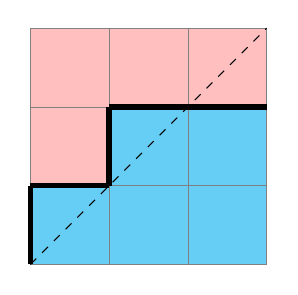
\begin{tikzpicture}
				\catalannumber{0,0}{3}{0,1,0,1,1};
			\end{tikzpicture}
			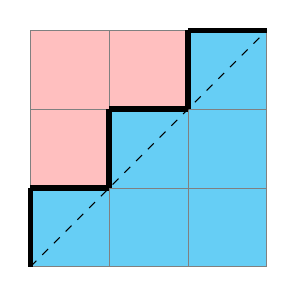
\begin{tikzpicture}
				\catalannumber{0,0}{3}{0,1,0,1,0,1};
			\end{tikzpicture}
			\caption{DPs corresponding to monomials $y_2y_4y_5$ and $y_2y_4y_6$.}
		\end{figure}
	\end{example}
\end{definition}

\begin{definition}[Gr\"obner Basis]
	Fix a monomial order on $\field[y_1, \dots, y_n]$. Then, a finite subset $G = \{g_1, \dots, g_h\}$ of 
	some ideal $I \subseteq \field[y_1, \dots, y_n]$, where $I$ is not the zero ideal, then $G$ is a 
	Gr\"obner basis if $\langle \text{LT}(g_i): g_i \in G \rangle = \langle \text{LT}(I) \rangle$. 
	In the case that $I = \{ 0\}$, then we will define the corresponding $G$ as empty set $\langle \emptyset \rangle$.
\end{definition}
\begin{definition}[Reduced Gr\"obner Basis]
	If some polynomial ideal $I$ has a Gr\"obner basis $G$ such that:
	\begin{itemize}
		\item LeadingConstant$(p) : p \in G = 1$
		\item $\forall p \in G, \text{monomials of }p \notin \langle \text{LT}(G \setminus   \{ p\}) \rangle$ 
	\end{itemize}
	Then $G$ is said to be a reduced Gr\"obner basis.
\end{definition}

\section{Constructing the Gr\"obner basis}

To construct the basis for $N = \field[y_1, \dots, y_n](y_1 + y_2 + \dots + y_n, y^2_1, y^2_2, \dots , y^2_n)$.
We will start by defining a set of \textit{Modified Catalan Paths} ($\alpha$) and the set $P_{\alpha}$ which will be used to characterize the polynomials in the Gr\"obner basis $G$ of $N$.

\begin{definition}[Modified Catalan Path ($\alpha$)] \label{alpha}
	Let us fix $n$ and let $n \in \mathbb{Z}^{+}$ and let $w$ be any Catalan path of length $2l \leq \lfloor n/2 \rfloor$, 
	such that $w \in \{0,1\}^{2l}$. Since, $w$ is a Catalan path the number of 1's = 0's, such that the number of 
	ones in $w$, $|w|_1 = l$ and the number of zeroes in $w$, $|w|_0 = l$.  Then let $\alpha = w 1(0)^m \in \{0,1\}^n$ which will be referred to as a modified Catalan path, where $m = n - d$ and $d = 2l + 1$.
\end{definition}


\begin{definition}[$P_{\alpha}$] \label{p_alpha}
	For a fixed modified Catalan path $\alpha$, define the set:
	\begin{align*}
		P_{\alpha} = \{ \beta = \beta_1 \cdots \beta_n \ | \ 1 \leq i \leq d, (\alpha_i = 0 \implies
		\beta_i = 0), |\alpha|_1 = |\beta|_1 \wedge \beta \neq \alpha \}
	\end{align*}
	Hence, this set $P_{\alpha}$ will contain all the MCPs that lie strictly above the path $\alpha$, since
	$\alpha$ is the representation for the leading terms in $G$. In other words, $P_{\alpha}$ contains
	the bit-string representation of the trailing monomials for each leading term $\alpha \in G$.
\end{definition}
\begin{remark}
    Note that $\alpha >_{lex} \beta$,  $\forall \beta \in P_{\alpha}$. Since, $\alpha$ represents the leading terms of $G$ 
    and the $\beta$ represent the trailing monomials for the fixed $\alpha$.
\end{remark}

\begin{proposition}
	\label{g_alpha_prop}
	We claim that the reduced Gr\"obner basis $G$ of $I$ contains polynomials of the following form:
	\begin{equation}
		\tag{\ref*{g_alpha_prop}}
		g_{\alpha} = y^{\alpha} + \sum_{\beta \in P_{\alpha}} y^{\beta}
	\end{equation}
	In other words, we will show that $g_\alpha \in \ideal$. 
\end{proposition}

To show \ref{g_alpha_prop} we must first understand how $g_{\alpha} \in G$ are generated. In other words, we must understand which S-polynomials are important and
	meaningful to compute such that the set of all such S-polynomials modulo some intermediate ideal, gives us the complete reduced Gr\"obner basis
	$G$ for $I$.

\begin{definition}[$P^{(k)}_{\alpha}$] \label{p_alpha_k}
	We define the proper subset:
	\begin{align*}
		P_\alpha^{(k)} = \{\beta = \beta_1 \cdots \beta_n \in P_\alpha \ | \ \beta_k = 0\} \subsetneq P_\alpha
	\end{align*}
	Hence, $P_\alpha^{(k)}$ consists of all paths $\beta \in P_\alpha$ that have a \texttt{0} at the 
	$k^{th}$ entry. 
\end{definition}

\begin{proposition} 
	\label{spoly_prop}
	Let the initial ideal $F_0 = (y^2_1, \dots, y^2_n)$. Then we claim the final reduced Gr\"obner basis $G$ 
	is given by the S-polynomials of the form:
	\begin{equation}
		\tag{\ref*{spoly_prop}}
		\overline{S(g_\alpha, y^2_k)}^{F_0} = \sum_{\beta \in P^{(k)}_{\alpha}} y^{\beta}y_k
	\end{equation}
	Where $\alpha$ contains a \texttt{1} in the $k^{th}$ position; otherwise, the reduction goes to \texttt{0} as the leading terms will be relatively prime by theorem 4 in \cite[\S 2.9]{iva}. 
\end{proposition}

\begin{proof} 
	We will prove \ref{spoly_prop} by induction on $l$, where $|w|_1 = l$. 
	\subsection*{Base Case} $l = 0$ then we know that $|\alpha|_1 = l + 1 = 1$:
	\begin{align*}
		\overline{S(g_{\texttt{1}}, y^2_1)}^{F_0} &= y_1g_{\texttt{1}} - y^2_1 \\
										  &= y_1(y_1 + y_2 + \dots + y_n) - y^2_1 \\
										  &\overset{\mathclap{\strut \mod F_0}} = \hspace{1 em} y_1y_2 + y_1y_3 + \dots + y_1y_n
	\end{align*}
	Since, $P^{(1)}_{1} = \{ y_2, \dots, y_n\}$ we have:
	\begin{equation*}
		\overline{S(g_{\texttt{1}}, y^2_1)}^{F_0} = \sum_{\beta \in P^{(1)}_{1}} y^{\beta}y_1
	\end{equation*}
	Now we will assume this result holds for $l$ and prove it for $l+1$. 
	\subsection*{Inductive Step} $l = l+1$: \\
	Let a modified Catalan path $\zeta$ have $l + 2$ ones such that $\zeta_{k} = 1$. \\ 
	\textbf{Case 1}. $\text{LM}(g_\zeta), y_k^2$ are not \textit{relatively prime}: 
	\begin{align*}
		\text{LCM}(\text{LM}(g_\zeta), y_k^2) 	&= y^{\zeta} y_k \\
		\overline{S(g_{\zeta}, y^2_k)}^{F_0} 	&= \frac{y^{\zeta} y_k}{y^\zeta} g_{\zeta} - \frac{y^{\zeta} y_k}{y^2_k} y^2_k \\
										  		&= y_k(g_{\zeta}) - y^{\zeta} y_k \\
												&= y_k(y^{\zeta} + g_{\beta}) - y^{\zeta} y_k \\
												&= y^{\zeta - k} y^2_k + g_{\beta}y_k - y^{\zeta-k} y_k^2 \\
												&= g_{\beta}y_k
	\end{align*}
	\textbf{Case 2}. $\text{LM}(g_\zeta), y_k^2$ are \textit{relatively prime}: \\
	To prove this, we will assume LC$(g_\zeta)$ = LC$(y^2_k) = 1$. Then, let $g_\zeta = y^{\zeta} + g_\beta$, where 
	LM$(g_\zeta) = y^{\zeta}$.
	\begin{align*}
		\text{LCM}(\text{LM}(g_\zeta), y_k^2) 	&= y^{\zeta}y^2_k \\
		\overline{S(g_{\zeta}, y^2_k)}^{F_0} 	&= \frac{y^{\zeta}y^2_k}{y^{\zeta}} g_{\zeta} - \frac{y{\zeta}y^2_k}{y^2_k} y^2_k \\
												&= y^2_k(y^{\zeta} + g_{\beta}) - y^{\zeta}y^2_k \\
												&\overset{\mathclap{\strut \mod F_0}} = \hspace*{1em} 0
	\end{align*}
\end{proof}



\section{Proving $G$ is a Reduced Gr\"obner Basis}
To prove \ref{g_alpha_prop} we will do a proof by induction. So far, we understand that \ref{spoly_prop} is used to generate new terms in the 
intermediate ideal which will eventually be a reduced Gr\"obner basis. The S-polynomial that we compute also have to go thorough a set of reductions 
with respect to some intermediate ideal. To show that \ref{spoly_prop} holds, we must also understand how the S-polynomials are reduced. 

	We will show \ref{g_alpha_prop} for all $n$, by induction on $l$, where $|w|_1 = l$.
	\subsection*{Base Case} $l = 0$: \\
	If $l = 0$ then we know that $|\alpha|_1 = l + 1 = 1$. \\ 
	Then we have $F_l = \langle y^2_1, y^2_2, \dots, y^2_n \rangle$ with $\alpha = 01(0)^m$, such that:
	\begin{align*}
		g_{\texttt{1}} &= y_1 + y_2 + \dots + y_n \\
		g_{\texttt{1}} &= y_1 + \sum_{\beta \in P_{1}^{(1)}} y^{\beta}
	\end{align*}
	Hence, we have verified the base case is true. Now, we will assume the result holds for for all $\alpha = w1(0)^m$ 
	with any Catalan path of length $x \leq l$ for a fixed $l$ and show that it holds for $l+1$. 
	\subsection*{Inductive Step} $l = l + 1$: \\
	Firstly, for a fixed $n$, if the value for $l+1 > \lfloor n/2 \rfloor$, then $g_{\alpha} = 0$, since $2l < \lfloor n/2 \rfloor$
	and once we substitute $l = l + 1$ we see that $2(l+1) \leq \lfloor n/2 \rfloor$. Hence, to prove this step of the result we need 
	to understand $all$ possible S-polynomials from the current set of $g_{\alpha}$ that we have so far.

	let us define $F_l$:
	\begin{equation*}
		F_l = \{ y^2_1, y^2_2, \dots, y^2_n\} \cup \{ g_{\alpha} \ | \ \alpha = w1 \in \{0,1\}^{2l+1} \}
	\end{equation*}

	Now we will examine three classes of S-polynomials and explore their reduction.
	
	\begin{lemma}[$\overline{S(g_{\alpha}, y^2_k)}^{F_l} = 0$] \label{lem_spoly_prime}
	If there is a zero in the $k^{th}$ position of $\alpha$, then it follows that LT($g_{\alpha}$) and $y^2_k$ 
	are relatively prime.
	\end{lemma}
	\begin{proof}
		Already shown in the proof of \ref{spoly_prop}.
	\end{proof}
	

	\begin{lemma}
		For some $k$ in the position of any $\alpha_i$, such that $\alpha_k = 1$, it follows that $|\alpha|_1 = l+1$. Let \textcolor{blue}{$\phi$} denote linear equivalence. Then, 
		we will show that:
		\begin{figure*}[hbt!]
			\begin{tikzcd}[column sep = 1em]
				\overline{S(g_{\alpha}, y^{2}_{k_1})}^{F_l} \ar[d, leftrightarrow, blue, "\phi" description] \ar[r, red]	& \overline{S(g_{\alpha}, y^{2}_{k_2})}^{F_l} \ar[d, leftrightarrow, blue, "\phi" description] \ar[r, red] 	& \cdots	\ar[d, leftrightarrow, blue, "\phi" description] \ar[r, red] & \overline{S(g_{\alpha}, y^{2}_{k_{l+1}})}^{F_l} \ar[d, leftrightarrow, blue, "\phi" description] \\
				g_{\alpha^{(k_1)}} \ar[r, red]																		& g_{\alpha^{(k_2)}} 						  						 \ar[r, red]							& \cdots	 						\ar[r, red]						  & g_{\alpha^{(k_{l+1})}}
			\end{tikzcd}
		\end{figure*} 
	\end{lemma}
	
We will analyze the set of paths produced after computing the appropriate S-polynomials and show that $g_{\alpha^{k_j}}$ is 
	linearly equivalent to $S_{k_j}$.
	\begin{remark}
		$\alpha^{(k_j)}$ denotes a string $\alpha\texttt{1}$ with the $k^{th}$ position replaced by a 0 (since it was a 1
		before). Any Catalan path can be obtained in this manner. Also note that if $2l + 1 \geq n$ the resulting
		S-polynomial mod $F_l$ will be 0.
	\end{remark}

	\subsection*{Graphical Representation} 
	First, assume that $n > 2l+1$ (non-trivial case). Note that for any $\beta \in P_\alpha^{(k)}$, $\beta_k =0$. Now define the $L_{k}$ as the diagonal line with a slope of $-1$ intersecting through the $k^{th}$ position of $\alpha$, and $L_d$ as the diagonal line with a slope of $-1$
	intersecting the $d^{th}$ position of $\alpha$ (the last $1$ in $\alpha$). Then any such $\beta$ must have a $0$ (north step) ending at some position on the line $L_k$ and \textit{cannot end} on any position in $L_d$.
	\begin{example} \label{p_alpha_k_exmaple}
		Suppose, $k=4$, and $\alpha = \texttt{01011}$ then it has the following bit-string and graphical representation: \vspace*{-1 em}
		\begin{figure}[h!] %
			\centering
			\begin{subfigure}{0.45\linewidth}
				\begin{align*}
					P^{(4)}_{ \color{red} \alpha} = \begin{cases}
						\texttt{01001} | \cdots \texttt{1} \cdots \cdots \cdots\\
						\texttt{01000} | \cdots \texttt{1} \cdot \texttt{1} \cdots \cdots \\
						\texttt{00001} | \cdots \texttt{1} \cdot \cdot \texttt{1} \cdots \cdots \\
						\texttt{00000} | \cdots \texttt{1} \cdots \texttt{1} \cdot \cdot \texttt{1} \cdots
					\end{cases}
				\end{align*}
			\end{subfigure}
			\qquad
			\begin{subfigure}{0.45\linewidth}
				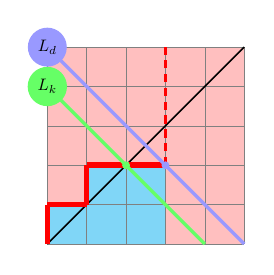
\begin{tikzpicture}[scale=0.5]
					%\catalannumber{0,0}{4}{0,1,0,1,0,1};
					\myfigone{0,0}{5}{0,1,0,1,1}{2}{3};
				\end{tikzpicture}
				%\hspace*{2em}
			\end{subfigure}
			\caption{The set of paths in $P^{(4)}_{\color{red} \alpha}$ and a graphical representation of \textcolor{red}{$\alpha$}}
		\end{figure}
		
		\begin{figure}[h!] %
			\centering
			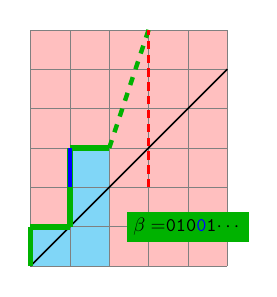
\begin{tikzpicture}[scale=0.5]
		            \palphak{0,0}{5}{0,1,0,0,1}{2}{3};
	            \end{tikzpicture}
	            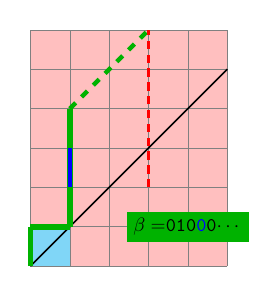
\begin{tikzpicture}[scale=0.5]
		            \palphakk{0,0}{5}{0,1,0,0,0}{2}{4};
	            \end{tikzpicture}
	       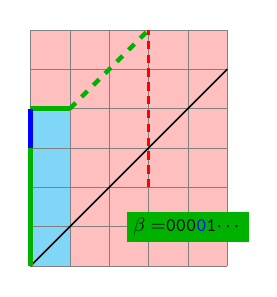
\begin{tikzpicture}[scale=0.5]
					\palphakkk{0,0}{5}{0,0,0,0,1}{2}{3};
			\end{tikzpicture}
			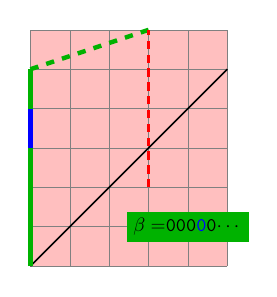
\begin{tikzpicture}[scale=0.5]
				\palphakkkk{0,0}{5}{0,0,0,0,0}{2}{4};
			\end{tikzpicture}
			\caption{Graphical representation of the set of paths in $P^{(4)}_{\color{red} \alpha}$}
		\end{figure}
		
		
	\end{example}
	
From example \ref{p_alpha_k_exmaple}, it is evident that all $\beta \in P^{(4)}_{\alpha}$ must have an upward step ending on the line $L_k$. This implies that $\beta$ is determined by the first $d$ entries, and everything following it is `free' (i.e. no restrictions other than number of ones). Also note that the number of zeros in $\beta_1 \cdots \beta_d$  determines the position of $\beta$ on the line $L_d$. We will denote:
\begin{equation*}
	| \beta_1 \cdots \beta_d|_0 = q
\end{equation*}
It follows that by complementary property of the bit string, we can count the number of ones in the first $d$ entries as well:
\begin{equation*}
	|\beta_1 \cdots \beta_d |_1 = l + 1 - q 
\end{equation*}
Where $|\beta|_1 = l + 1$ by definitions \ref{p_alpha} and \ref{p_alpha_k}.
\subsection*{Partitioning the Paths}
\begin{definition}[$U_{\alpha}$ Paths] \label{u_alpha}
	For a fixed $\alpha$, define the set:
	\begin{equation}
		U_{\alpha} = \{ u = u_1 \cdots u_d \ | \ \alpha_i = 0 \implies u_i = 0,1 \leq i \leq d \wedge u \neq \alpha \} 
		\tag{\ref*{u_alpha}}
	\end{equation}
\end{definition}

\begin{definition}[$P_{u, \alpha}$ Paths] \label{p_u_alpha}
	For a fixed $u \in U_{\alpha}$, define the subset of $P_\alpha$ as:
	\begin{equation}
		P_{u, \alpha} = \{ \beta = u \beta_{d+1} \cdots \beta_n \ |   \ |\beta|_1 = l+1\} \subsetneq P_\alpha
		\tag{\ref*{p_u_alpha}}
	\end{equation}
\end{definition}

\begin{example} \label{u_alpha_example}
	If $\alpha = \texttt{010110} \cdots \texttt{0}$, we have $d=5$ so:
	\begin{equation*} 
		U_{\texttt{010110} \cdots \texttt{0}} = \{\texttt{01010, 01001, 01000, 00011, 00010, 00001, 00000}\}
	\end{equation*}
\end{example} 
Since each subset $P_{u, \alpha}$ is disjoint, we can partition $P_\alpha$ into subsets of bit-strings that start with a particular $u \in U_\alpha$ (and end in the appropriate manner):
\begin{equation} \label{p_alpha_union}
	P_\alpha = \bigcup_{u \in U_\alpha} P_{u,\alpha} \tag{\ref*{u_alpha_example}.1}
\end{equation}
By the above, we can separate the sum of polynomials in $P_\alpha$ algebraically:
\begin{align*} \label{y_beta_sum}
	\sum_{\beta \in P_\alpha} y^ \beta  &= \sum_{u \in U_\alpha} \  \sum_{\beta \in P_{u,\alpha}} y^\beta \\ 
										&= \sum_{r=1}^{l+1} \sum_{u^{(r)} \in U_\alpha} y^{u^{(r)}} 
										\sum_{d+1 \leq i_1 < \cdots < i_r \leq n} y_{i_1} \cdots y_{i_{r}}   
										\tag{\ref*{u_alpha_example}.2}
\end{align*} 
Where $u^{(r)}$ is some $u \in U_\alpha$ such that  $|u^{(r)}|_1  = l + 1 -r$; in other words, for a given $u \in U_\alpha$, it's latter portion $\beta_{d+1} \cdots \beta_{n}$ has $r$ ones; these monomials $y_{i_1} \cdots y_{i_r}$ are the `free' portion in the latter part of the path $\beta$ as described in the graphical section.

\begin{remark}
	Observe that by Claim 1.1, we need only consider bit strings in $P_{\alpha}^{(k)}$, so we will develop analogous notation and definitions to \ref{u_alpha}-\ref{y_beta_sum}.
\end{remark}

\begin{definition}[$U^{(k)}_{\alpha}$] \label{u_alpha_k}
	For a fixed $\alpha$, define the set:
	\begin{equation}
		U_\alpha^{(k)} = \{u \in U_\alpha \ | \ u_k = 0 \} \subsetneq U_\alpha \tag{\ref*{u_alpha_k}}
	\end{equation}
\end{definition}
\begin{definition}[$P_{u,\alpha}^{(k)}$] \label{p_u_alpha_k}
	For a fixed $u \in U_\alpha^{(k)}$, define the set:
	\begin{equation}
		P_{u,\alpha}^{(k)} = \{\beta = u \beta_{d+1} \cdots \beta_n \ | \ |\beta|_1 = l + 1 \} \subsetneq P_{u,\alpha} \tag{\ref*{p_u_alpha_k}}
	\end{equation}	
\end{definition}

By the new analogous notation and definitions we can state the partition of \ref*{p_alpha_union} as:
\begin{equation*}
	P_\alpha^{(k)} = \bigcup_{u \in U_\alpha^{(k)}} P_{u,\alpha}^{(k)} \tag{\ref*{p_u_alpha_k}.1}
\end{equation*}
Then by \ref{spoly_prop}, we can state:
\begin{align} 
	\overline{S(g_\alpha, y_k^2)}^{F_0} = \sum_{\beta \in P_\alpha^{(k)}} y^\beta y_k  = \sum_{r=1}^{l+1}\sum_{u^{(r)} \in U_\alpha^{(k)}} y^{u^{(r)}}y_k \sum_{d+1 \leq i_1 < \cdots < i_r \leq n} y_{i_1} \cdots y_{i_{r}}  \tag{\ref*{p_u_alpha_k}.2}
\end{align}
Where each $u^{(r)} \in U_\alpha$ such that $|u^{(r)}|_1 = l + 1 - r$. 



























	
	
% 1/2 Property b) + c) (Xavier)
\clearpage


\subsection*{Special Paths}

\begin{definition} \label{uprimes}
For a fixed $k \in \Z ^+$, define $u' \in U_\alpha^{(k)}$ as an element such that:

\begin{align*}
    u'_j = \alpha_j \\
\end{align*}

For all $j \ne k$ on $1 \leq j \leq d$ where $u'_k = 0$. Therefore we can write:

\begin{align*}
u' = \alpha_1 \cdots \alpha_{k-1} 0 \alpha_{k+1} \cdots \alpha_d    \in U_\alpha^{(k)} \\
\end{align*}

\end{definition}


\begin{definition} \label{bprimes}
For a fixed $k \in \Z ^+$ and for a fixed $u' \in U_\alpha^{(k)}$, define $\beta' \in P_\alpha^{(k)}$ as an element such that:

\begin{align*}
    \beta' = u' \beta_{d+1} \cdots \beta_n \in P_\alpha^{(k)} \\
\end{align*}

\end{definition}





\begin{example} \label{bprime_before}
    $\beta'$ Alone (graph placeholder)
\end{example}



Notice that $\beta'$ follows the path of $\alpha$ until the $k^{th}$ position, since there must be a movement North to the line $L_k$ by the definition of $P_\alpha^{(k)}$; $\beta'$ subsequently `mirrors' $\alpha$ until the $d^{th}$ entry $\beta_d$, after which $\beta_{d+1} \cdots \beta_n$ consists of non-fixed entries that vary depending on which $\beta'$ is selected for a fixed $u'$. 



\begin{remark} \label{bprime_ones}
    Also note that $|u'|_1 = l$, since $|\alpha|_1 = l+1$ and only $u_k \ne \alpha_k$ with all other entries equal. Therefore, the variable entries $\beta_{d+1} \cdots \beta_n$ contain only one entry with $\beta_{t} = 1$ for some $d+1 \leq t \leq n$ given by the restriction $|\beta'|_1 = l+1$.
\end{remark}



\begin{example} \label{bprime_after}
    $\beta'$ After Multiplication (graph placeholder)
\end{example}
Notice that the graph of $\beta'$ from $\beta_k \cdots \beta_{n}$ has been translated down by one unit and translated to the right by one unit. 


\begin{remark} \label{bprime_equiv}
    By \ref{bprime_ones}, we can write $y^{\beta'} = \frac{y^\alpha}{y_k}y_j$ for some $j$ bounded on $d+1 \leq j \leq n$. It follows that:
    
    \begin{align*}
        y^{\beta'}y_k &= \Big(\frac{y^\alpha}{y_k}y_j\Big)y_k \\ 
        &= y^\alpha y_j \\
    \end{align*}
    
For some $j$ on $d+1 \leq j \leq n$.
\end{remark}








\subsection*{Reductions}

We begin by breaking apart the partially reduced S-polynomial from \ref{spoly_prop} with:

\begin{align*}
    \overline{S(g_\alpha, y_k^2)}^{F_0} = \sum_{\beta \in P_\alpha^{(k)}}y^\beta y_k  = \sum_{\beta ' \in P_\alpha^{(k)}} y^{\beta'} y_k + \sum_{\beta \in P_\alpha^{(k)}, \beta \ne \beta '} y^\beta y_k \\
\end{align*}

Observe the term on the left consisting of all $\beta'$ for a fixed $\alpha$. Using \ref{bprime_equiv}, we state:

\begin{align*}
    \sum_{\beta ' \in P_\alpha^{(k)}} y^{\beta'} y_k &= \sum_{j=d+1}^n y^\alpha y_j \\
\end{align*}

This follows from the fact that the variable entries $\beta_{d+1} \cdots \beta_n$ will only have one entry with $\beta_t = 1$; thus, if we sum over all such $\beta'$ we arrive at the expression above. 


\begin{remark} \label{bprime_decon}
    Since the leading term of the sum above contains a monomial factor of $\text{LT}(g_\alpha) = y^\alpha$, then by the Division Algorithm on lex order we can reduce the expression further $\text{mod} \ g_\alpha$:
    \begin{align*}
     \sum_{\beta ' \in P_\alpha^{(k)}} y^{\beta'} y_k &\equiv \sum_{j=d+1}^n y^\alpha y_j \\
     &\equiv \sum_{j=d+1}^n y^\alpha y_j - g_\alpha \sum_{j=d+1}^n y_j \\ 
    &\equiv \sum_{j=d+1}^n y^\alpha y_j - \Big(y^\alpha + \sum_{\gamma \in P_\alpha}y^\gamma\Big) \sum_{j=d+1}^n y_j \ \tag{\text{by the Inductive Hypothesis}} \\ 
    &\equiv  -\sum_{\gamma \in P_\alpha}y^\gamma \sum_{j=d+1}^n y_j \\ 
    & \equiv - \sum_{v \in U_\alpha} \sum_{\gamma \in P_{v,\alpha}}y^\gamma \sum_{j=d+1}^n y_j \tag{by Partition of $P_\alpha$} \\
\end{align*}
And recall by 3.10.2 of \ref{p_u_alpha_k}, we can further deconstruct this sum to:

\begin{align*}
      \sum_{\beta ' \in P_\alpha^{(k)}} y^{\beta'} y_k \equiv - \sum_{r=1}^{l+1} \sum_{v^{(r)} \in U_\alpha} y^{v^{(r)}}\sum_{d+1 \leq i_1 < \cdots < i_r \leq n}y_{i_1} \cdots y_{i_r} \sum_{j=d+1}^n y_j\\
\end{align*}

\pagebreak

Expanding the sum on the right gives us:

\begin{align*}
    \sum_{\beta ' \in P_\alpha^{(k)}} y^{\beta'} y_k \equiv - \sum_{r=1}^{l+1} \sum_{v^{(r)} \in U_\alpha} y^{v^{(r)}} (r+1) \sum_{d+1 \leq i_1 < \cdots < i_{r+1} \leq n}y_{i_1} \cdots y_{i_r} y_{i_{r+1}} \\
\end{align*}

\end{remark}

This results from the following observation. Suppose we examine the product of:

\begin{align*}
    (y_{i_1} \cdots y_{i_r})(y_j), \ \ \text{for some} \ d+1 \leq j \leq n \\
\end{align*}

Then either $j = i_t$ for some $1 \leq t \leq r$, which will result in a monomial with a squared factor $y_j^2$ and thus reduced to zero modulo $F_l$; or $j \ne i_t$ for all $1 \leq t \leq r$, resulting in a monomial with no squared variables. Because we have $d+1 \leq i_1 < \cdots < i_{r+1} \leq n$, then for any $y_j y_{i_1} \cdots y_{i_r}$, there exists an equal monomial $y_{i_1'} y_{j'} \cdots y_{i_r'}$, where $i_1' = j$ and $j' = i_1$. We can continue this process for all possible positions of $j$, which will give us $(r+1)$ ways of writing the same monomial. Therefore, for each unique monomial received from the expansion, it will have a coefficient of $(r+1)$.


	
	
	
	
	


\newpage
%-------------------------------------------------------------------
% Begin BIBLIOGRAPHY
%-------------------------------------------------------------------

\small
%\bibliographystyle{abbrv}  
\bibliographystyle{amsalpha}  
%\bibliographystyle{plain}  
%\bibliographystyle{amsplain}  
%\bibliography{AntipodeLinHopfMono}
\bibliography{refrences}
\end{document}
